\ifdefined\ishandout
\documentclass[handout]{beamer}
\else
\documentclass{beamer}
\fi

\usepackage[frenchb]{babel}
\usepackage[T1]{fontenc}
\usepackage[latin1]{inputenc}
\usepackage{hyperref}
\usepackage{multirow}
\usepackage{listings}
\usepackage{fancyvrb}
\usepackage{tikz}
\usepackage{framed}
\usepackage{algorithm}
\usepackage{algorithmic}
\usepackage{xcolor}
\usepackage{booktabs}
\usepackage{color, colortbl}
\ifdefined\ishandout
\usepackage{handoutWithNotes}
\fi
\usepackage{slashbox}
\usepackage{amsmath}
\usepackage{bm}
\usepackage{hhline}

\usetikzlibrary{shapes.geometric}
\usetikzlibrary{positioning}
\usetikzlibrary{shapes.arrows, chains}
\usetikzlibrary{arrows,calc}
\usetikzlibrary{shapes.multipart}
\usepackage{array}
\usetheme{Boadilla}

\usefonttheme[onlymath]{serif}

\newcommand{\R}{\mathbb{R}}
\newcommand{\C}{\mathbb{C}}
\newcommand{\N}{\mathbb{N}}
\newcommand{\Z}{\mathbb{Z}}
\newcommand{\E}{\mathbb{E}}
\newcommand{\Var}{\text{Var}}
\newcommand{\Cov}{\text{Cov}}
\ifdefined\ishandout
\pgfpagesuselayout{3 on 1 with notes}[a4paper,border shrink=5mm]
\usecolortheme{dove}
\else
%\usecolortheme{dolphin}
\usecolortheme{beaver}
\fi


\lstnewenvironment{codeC}
{ \lstset{language=C,
    otherkeywords={printf,scanf}}
}
{}

\ifdefined\ishandout
\definecolor{mygreen}{rgb}{0,0,0}
\definecolor{mymauve}{rgb}{0,0,0}
\definecolor{myblue}{rgb}{0,0,0}
\else
\definecolor{mygreen}{rgb}{0,0.6,0}
\definecolor{mymauve}{rgb}{0.58,0,0.82}
\definecolor{myblue}{rgb}{0,0,1}

\fi

%% Notes
%\setbeameroption{show only notes}


\definecolor{mygray}{rgb}{0.5,0.5,0.5}

\lstset{ language=Python,%
  backgroundcolor=\color{white},   % choose the background color; you must add \usepackage{color} or \usepackage{xcolor}
  basicstyle=\footnotesize,        % the size of the fonts that are used for the code
  breakatwhitespace=false,         % sets if automatic breaks should only happen at whitespace
  breaklines=true,                 % sets automatic line breaking
  captionpos=b,                    % sets the caption-position to bottom
  commentstyle=\color{mygreen},    % comment style
  deletekeywords={...},            % if you want to delete keywords from the given language
  escapeinside={\%*}{*)},          % if you want to add LaTeX within your code
  extendedchars=true,              % lets you use non-ASCII characters; for 8-bits encodings only, does not work with UTF-8
  frame=tb,	                   % adds a frame around the code
  keepspaces=true,                 % keeps spaces in text, useful for keeping indentation of code (possibly needs columns=flexible)
  keywordstyle=\color{blue},       % keyword style
  otherkeywords={*,...},           % if you want to add more keywords to the set
  numbers=none,                    % where to put the line-numbers; possible values are (none, left, right)
  numbersep=5pt,                   % how far the line-numbers are from the code
  numberstyle=\tiny\color{mygray}, % the style that is used for the line-numbers
  rulecolor=\color{black},         % if not set, the frame-color may be changed on line-breaks within not-black text (e.g. comments (green here))
  showspaces=false,                % show spaces everywhere adding particular underscores; it overrides 'showstringspaces'
  showstringspaces=false,          % underline spaces within strings only
  showtabs=false,                  % show tabs within strings adding particular underscores
  stepnumber=2,                    % the step between two line-numbers. If it's 1, each line will be numbered
  stringstyle=\color{mymauve},     % string literal style
  tabsize=3,	                   % sets default tabsize to 2 spaces
  title=\lstname                   % show the filename of files included with \lstinputlisting; also try caption instead of title
}
%\lstset{language=Python,
% breakatwhitespace=false,         % sets if automatic breaks should only happen at whitespace
%  breaklines=true,                 % sets automatic line breaking
%  captionpos=b,                
%%commentstyle=\itshape\color{mymauve},
%%keywordstyle=\bfseries\color{myblue},
%numbers=left,                    % where to put the line-numbers; possible values are (none, left, right)
%  numbersep=8pt,                   % how far the line-numbers are from the code
%  numberstyle=\tiny\color{mygray}, % the style that is used for the line-numbers
%%  rulecolor=\color{black},         % if not set, the frame-color may be changed on line-breaks within not-black text (e.g. comments (green here))
%  showspaces=false,                % show spaces everywhere adding particular underscores; it overrides 'showstringspaces'
%%  showstringspaces=false,          % underline spaces within strings only
%  showtabs=false,                  % show tabs within strings adding particular underscores
%  stepnumber=2,                    % the step between two line-numbers. If it's 1, each line will be numbered
%%  stringstyle=\color{mygreen},     % string literal style
%  tabsize=2 
%}
\ifdefined\ishandout
\newcommand{\red}{\textbf}
\else
\newcommand{\red}{\textcolor{red}}
\fi
%\newcommand \emph
%Default size : 12.8 cm * 9.6 cm

\newcommand{\tmark}[1]{\tikz[remember picture, baseline=-.5ex]{\coordinate(#1);}}

\ifdefined\ishandout
\newenvironment<>{codeblock}[1]{%begin
  \setbeamercolor{block title}{fg=black,bg=lightgray!80}%
  \begin{block}{#1}}
  % \begin{codeC}}
  %  {\end{codeC}
{  
\end{block}}

\newenvironment<>{termblock}[1]{
    \setbeamercolor{block title}{fg=black,bg=lightgray!90}%
    \begin{block}{#1}
}
%     \begin{Verbatim}}
{%\end{Verbatim}
\end{block}
}

\definecolor{bluegreen}{RGB}{0,0,0}
%\definecolor{bluegreen}{rgb}{0,0.6,0.8}
\else

\newenvironment<>{codeblock}[1]{%begin
  \setbeamercolor{block title}{fg=darkgray,bg=yellow}%
  \begin{block}{#1}}
  % \begin{codeC}}
  %  {\end{codeC}
{  
\end{block}}

\newenvironment<>{termblock}[1]{
    \setbeamercolor{block title}{fg=white,bg=lightgray}%
    \begin{block}{#1}}
%     \begin{Verbatim}}
{%\end{Verbatim}
\end{block}
}

\definecolor{bluegreen}{RGB}{0,149,182}
%\definecolor{bluegreen}{rgb}{0,0.6,0.8}
\fi

%\newcommand{\output}[1]{
\setbeamertemplate{navigation symbols}{}
\newcommand{\bvrb}{\Verb[commandchars=£µ§,formatcom=\color{bluegreen}]}
\newcommand{\footvrb}{\footnotesize\Verb}
\newcommand{\vrbalert}[2][]{\visible<#1>{#2}}
%%% Commande pour les listes/arbres
\newcommand{\mvide}{\nodepart{one} \nodepart{two}}
\newcommand{\tvide}{\nodepart{one} \nodepart{two} \nodepart{three}}

%%Fin des commandes pour les listes/arbres.



%%% Paramètres du cours (à régler)
%Numéro du cours
\newcommand{\nb}{1}

\title[non-linear]{Toward non-linear regression/classification}
\author[non-linear]{julien.brajard@upmc.fr}
\institute[UPMC]{UPMC}
\date{1-5 August 2016}
\begin{document}
%%%%%%%%%%%%%%%%%%%%% SLIDES DE TITRE
\begin{frame}
\titlepage
%\centering{
%\url{http://australe.upmc.fr} (onglet EPU-C5-IGE Info Gen)}
\end{frame}
%%%%%%%%%%%%%%%%%%%%%
\begin{frame}
\frametitle{Polynomial regression}
LInear regression
Polynome degree two
how to solve it ?
like linear regression
increasing the degree of the polynome ?
Values of coefficients ?
Idea of the regression
Ridge or Lasso
Ridge regression,
results for maxdeg 15 and different value of alpha
lasso regression
results for maxdeg 15 and different value of alpha
why it can be exactly zeros
model selection
learning/test/
validation
\end{frame}
\begin{frame}
\frametitle{Example of a non-linear relashionship}
\begin{figure}
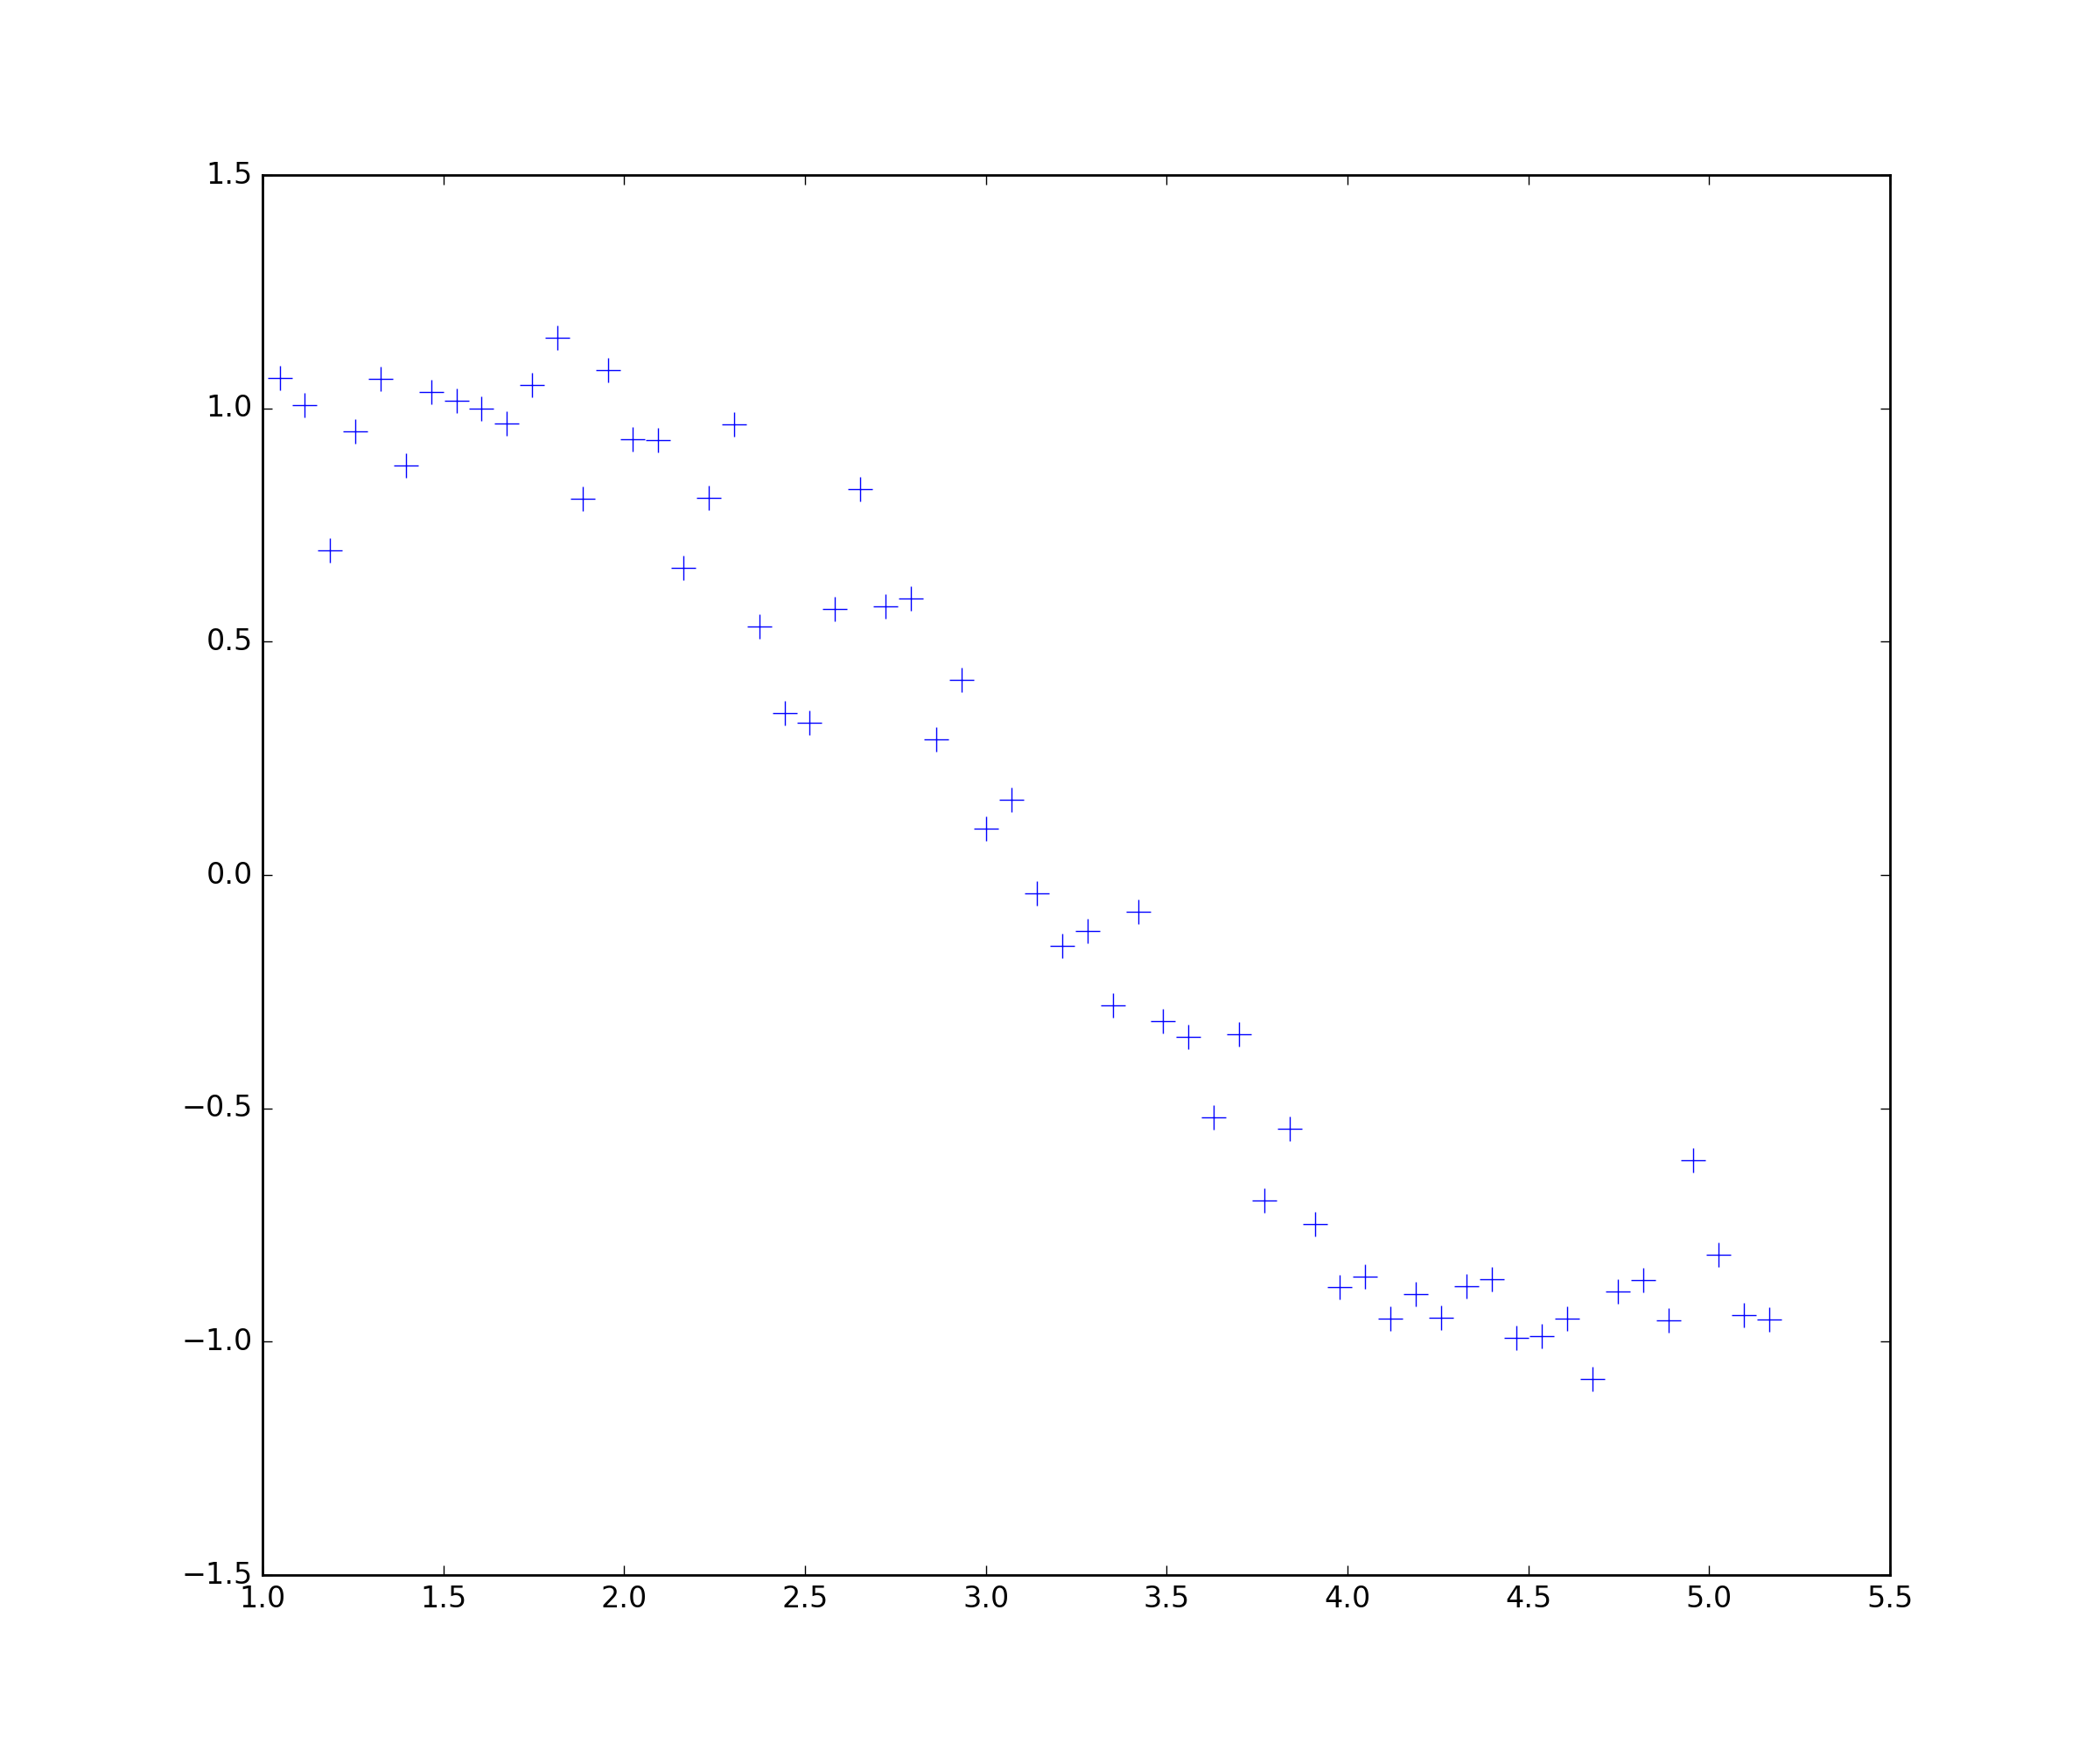
\includegraphics[height=0.55\textheight]{./fig/scatter.png}
\end{figure}
\begin{block}{An idea}
We could take an polynomial hypothesis model:
$$
h_{\bm{\theta}}(x) = \theta_0 x^0 + \theta_1 x^1 + \ldots + \theta_p x^p
$$
\end{block}
\end{frame}
%%%%%%%%%%%%%%%%%%%%%
\begin{frame}
\frametitle{Example}
$\{(x_1,y_1),\ldots,(x_n,y_n)\}$ is the learning dataset.

For a given polynom degree $p$, parameters $\bm{\theta}$ are determined minimizing the 
least-mean square cost function:
$$
J(\bm{\theta}) = \frac{1}{n} \sum (y_i - h_{\bm{\theta}}(x))^2
$$

\end{frame}

%%%%%%%%%%%%%%%%%%%%%
\begin{frame}
\frametitle{Increasing the polynomial degree ?}
\end{frame}

%%%%%%%%%%%%%%%%%%%%%
\begin{frame}
\frametitle{Polynomial regression as a linear regression}
\begin{table}
\resizebox{\textwidth}{!}{%
\begin{tabular}{lllllllllll}
\toprule
{} &      rmse &      th\_0 &      th\_1 &      th\_2 &      th\_3 &      th\_4 &      th\_5 &      th\_6 &      th\_7 &      th\_8 \\
\midrule
max\_pow\_1  & +5.47e-02 & +1.96e+00 & -6.20e-01 &       NaN &       NaN &       NaN &       NaN &       NaN &       NaN &       NaN \\
max\_pow\_2  & +5.46e-02 & +1.91e+00 & -5.83e-01 & -5.96e-03 &       NaN &       NaN &       NaN &       NaN &       NaN &       NaN \\
max\_pow\_3  & +1.84e-02 & -1.08e+00 & +3.03e+00 & -1.29e+00 & +1.37e-01 &       NaN &       NaN &       NaN &       NaN &       NaN \\
max\_pow\_4  & +1.80e-02 & -2.66e-01 & +1.69e+00 & -5.32e-01 & -3.57e-02 & +1.39e-02 &       NaN &       NaN &       NaN &       NaN \\
max\_pow\_5  & +1.70e-02 & +2.99e+00 & -5.12e+00 & +4.72e+00 & -1.93e+00 & +3.35e-01 & -2.07e-02 &       NaN &       NaN &       NaN \\
max\_pow\_6  & +1.65e-02 & -2.80e+00 & +9.52e+00 & -9.71e+00 & +5.23e+00 & -1.55e+00 & +2.33e-01 & -1.36e-02 &       NaN &       NaN \\
max\_pow\_7  & +1.55e-02 & +1.93e+01 & -5.60e+01 & +6.90e+01 & -4.46e+01 & +1.65e+01 & -3.53e+00 & +4.05e-01 & -1.92e-02 &       NaN \\
max\_pow\_8  & +1.53e-02 & +4.32e+01 & -1.37e+02 & +1.84e+02 & -1.33e+02 & +5.77e+01 & -1.53e+01 & +2.42e+00 & -2.10e-01 & +7.68e-03 \\
max\_pow\_9  & +1.46e-02 & +1.68e+02 & -6.15e+02 & +9.63e+02 & -8.46e+02 & +4.61e+02 & -1.62e+02 & +3.68e+01 & -5.22e+00 & +4.22e-01 \\
max\_pow\_10 & +1.46e-02 & +1.38e+02 & -4.86e+02 & +7.26e+02 & -5.96e+02 & +2.93e+02 & -8.75e+01 & +1.45e+01 & -8.06e-01 & -1.38e-01 \\
max\_pow\_11 & +1.45e-02 & -7.49e+01 & +5.12e+02 & -1.33e+03 & +1.87e+03 & -1.61e+03 & +9.14e+02 & -3.50e+02 & +9.14e+01 & -1.61e+01 \\
max\_pow\_12 & +1.45e-02 & -3.39e+02 & +1.87e+03 & -4.42e+03 & +6.01e+03 & -5.25e+03 & +3.12e+03 & -1.30e+03 & +3.84e+02 & -8.03e+01 \\
max\_pow\_13 & +1.43e-02 & +3.20e+03 & -1.78e+04 & +4.46e+04 & -6.66e+04 & +6.61e+04 & -4.61e+04 & +2.32e+04 & -8.55e+03 & +2.30e+03 \\
max\_pow\_14 & +1.31e-02 & +2.38e+04 & -1.41e+05 & +3.79e+05 & -6.10e+05 & +6.57e+05 & -5.03e+05 & +2.82e+05 & -1.17e+05 & +3.66e+04 \\
max\_pow\_15 & +1.17e-02 & -3.62e+04 & +2.44e+05 & -7.46e+05 & +1.38e+06 & -1.71e+06 & +1.53e+06 & -1.00e+06 & +4.98e+05 & -1.88e+05 \\
\bottomrule
\end{tabular}
}
\end{table}
\end{frame}

%%%%%%%%%%%%%%%%%%%%%
\begin{frame}
\frametitle{Regularization}
\end{frame}

%%%%%%%%%%%%%%%%%%%%%
\begin{frame}
\frametitle{Learning/Validation dataset}
\end{frame}

%%%%%%%%%%%%%%%%%%%%%
\begin{frame}
\frametitle{Test dataset}
\end{frame}

%%%%%%%%%%%%%%%%%%%%%
\begin{frame}
\frametitle{Perceptron}
\end{frame}

%%%%%%%%%%%%%%%%%%%%%
\begin{frame}
\frametitle{}
\end{frame}

\end{document}